% ============================================================
% SPAGS: Spatial-aware Progressive Adaptive Gaussian Splatting
%        for Sparse-view Novel View Synthesis
% PG2026 Conference Paper
% ============================================================
\documentclass{egPublStyle}

\usepackage{graphicx}
\usepackage{booktabs}
\usepackage{amsmath}
\usepackage{amssymb}
\usepackage{multirow}
\usepackage{balance}
\usepackage{algorithm}
\usepackage{algpseudocode}

\title{SPAGS: Spatial-aware Progressive Adaptive Gaussian Splatting\\
       for Sparse-view Novel View Synthesis}

\author{
  Qiyu Hu\textsuperscript{1},
  Anonymous Author\textsuperscript{1}
  \vspace{4pt}\\
  \textsuperscript{1} School of Computer Science and Technology, XXX University
}

\conference{Pacific Graphics 2026}

\newcommand{\spags}{SPAGS}
\newcommand{\sps}{SPS}
\newcommand{\gap}{GAP}
\newcommand{\adm}{ADM}
\newcommand{\rtwo}{R\textsuperscript{2}-Gaussian}
\newcommand{\psnr}{PSNR}
\newcommand{\bdB}{dB}

\begin{document}

\maketitle

% ============================================================
\begin{abstract}
Sparse-view CT novel view synthesis aims to generate high-quality projection images from a limited number of X-ray exposures, reducing radiation dose while maintaining diagnostic quality. Existing 3D Gaussian Splatting methods for this task suffer from three key limitations: uniform initialization that ignores anatomical priors, gradient-based densification that creates excessive over-clustering in dense tissue regions, and spatially-agnostic density updates that cannot capture local tissue heterogeneity. We identify that the core challenge is not spatial sparsity---the conventional focus of few-shot 3DGS---but \textit{structural redundancy}: Gaussians proliferate at anatomical boundaries while under-representing uniform tissue regions.

To address this, we propose \spags, a progressive three-stage framework that introduces spatial awareness at each phase of the 3DGS pipeline. \textbf{\sps} leverages FDK reconstruction density priors for anatomically-guided Gaussian seeding (+0.21 dB). \textbf{\gap} performs proximity-guided pruning with gradient-aware filtering to remove redundant Gaussians in over-dense regions, delivering the dominant improvement (+0.42 dB). \textbf{\adm} introduces K-planes-based spatially-aware density modulation for fine-grained tissue-specific correction (+0.11 dB). On 5 organs across 2/3/4 projection views, \spags\ achieves 28.22 dB average PSNR at 3 views---outperforming \rtwo\ by +0.39 dB and surpassing other methods (CoR-GS, FSGS, X-Gaussian, DN-Gaussian) by 4--8 dB, while adding less than 10\% training overhead and zero inference cost.
\end{abstract}

% ============================================================
\section{Introduction}
\label{sec:intro}
% ============================================================

% --- Background ---
Novel view synthesis (NVS) from sparse observations is a critical challenge in computational imaging, with direct clinical implications for reducing radiation exposure in X-ray CT examinations. The central task is to generate high-quality projection images from arbitrary viewpoints given only a few input projections---a severely ill-posed inverse problem that requires strong priors for effective regularization.

3D Gaussian Splatting (3DGS)~\cite{kerbl20233d} has recently emerged as a powerful scene representation for radiance fields, offering real-time rendering with quality competitive with NeRF-based approaches. A 3DGS scene is represented as a collection of anisotropic 3D Gaussians, each parameterized by position $\boldsymbol{\mu} \in \mathbb{R}^3$, covariance $\boldsymbol{\Sigma} \in \mathbb{R}^{3\times3}$ (controlled via rotation $\mathbf{R}$ and scaling $\mathbf{S}$), opacity $\alpha \in [0,1]$, and spherical harmonic coefficients for view-dependent appearance. The differentiable rasterization pipeline renders these Gaussians via $\alpha$-blending, enabling efficient gradient-based optimization from multi-view images.

For CT imaging, \rtwo~\cite{hu2024r2} adapted this framework by replacing the standard $\alpha$-blending with a physically-motivated radiative transfer model based on the Beer-Lambert law:
\begin{equation}
I(\mathbf{u}) = I_0 \cdot \exp\left(-\sum_{i=1}^{N} \rho_i \cdot \ell_i(\mathbf{u})\right),
\label{eq:beer_lambert}
\end{equation}
where $I(\mathbf{u})$ is the intensity at pixel $\mathbf{u}$, $I_0$ is the source intensity, $\rho_i$ is the linear attenuation coefficient, and $\ell_i(\mathbf{u})$ is the ray segment length. This physically accurate forward model enables differentiable forward and backward projection, establishing a strong baseline for sparse-view CT NVS.

% --- Motivations ---
Despite these advances, existing 3DGS-based methods inherit three key limitations from forward-facing 3DGS that are particularly damaging for CT NVS.

\textit{Limitation 1: initialization bias.} Conventional 3DGS initializes Gaussians from an SfM point cloud or uniformly within the scene bounding box---methods that assume textured surfaces with feature correspondences. CT projection images, however, are attenuation integrals without identifiable features, causing SfM to fail and uniform initialization to distribute Gaussians indiscriminately throughout the volume. This wastes capacity on empty regions while undersampling anatomically important structures, and Gaussians that start far from anatomical features may never recover during optimization.

\textit{Limitation 2: ineffective densification.} The gradient-based densification mechanism---cloning Gaussians with large view-space position gradients---works well for forward-facing scenes where gradient signals clearly distinguish sparse from dense regions. In CT volumes, the entire space is densely occupied, making the gradient signal spatially diffuse. Critically, proximity-guided densification (FSGS~\cite{zhu2024fsgs}) designed for filling gaps in forward-facing scenes is counterproductive here: adding Gaussians to regions with large nearest-neighbor distances exacerbates already-severe over-clustering at anatomical boundaries.

\textit{Limitation 3: spatially-agnostic density updates.} All Gaussian density parameters share identical learning rules regardless of anatomical context. Two Gaussians representing bone (high attenuation) and soft tissue (low attenuation) receive the same gradient-based updates, preventing the model from learning that different anatomical regions have distinct density characteristics.

% --- Our insight ---
Our key insight is that these three limitations share a common root cause: the absence of explicit spatial reasoning in the 3DGS pipeline. CT volumes carry strong spatial priors (density varies predictably with anatomy) and exhibit structured geometric patterns (dense at boundaries, sparse within uniform tissue) that standard spatially-agnostic mechanisms cannot exploit. We address all three limitations through a unified principle---introduce spatial awareness at each critical decision point---resulting in the \spags\ framework.

% --- Our approach ---
Building on this insight, we propose \spags, a progressive three-stage framework that introduces spatial awareness at each phase of the 3DGS pipeline (Figure~\ref{fig:overview}).

\textbf{Stage 1: \sps.} Rather than initializing Gaussians uniformly, \sps\ leverages the FDK reconstruction volume---a standard filtered back-projection result available in any CT workflow at negligible computational cost---as a spatial prior for Gaussian seeding. While the FDK volume contains artifacts from sparse projections (streaking, blurring), it provides a coarse density map that roughly distinguishes anatomical regions. By sampling proportionally to FDK density values with a controlled uniform component, \sps\ concentrates initial Gaussians in anatomically relevant regions while ensuring basic coverage of low-density areas.

\textbf{Stage 2: \gap.} Standard 3DGS training with gradient-based densification on CT volumes creates excessive Gaussian clustering in high-density regions (bones, tissue boundaries), where many Gaussians compete to represent the same local structure. \gap\ addresses this by inverting the conventional wisdom of few-shot 3DGS: rather than adding Gaussians in sparse regions~\cite{zhu2024fsgs}, it removes redundant Gaussians in dense regions. For each Gaussian, \gap\ computes a proximity score based on the mean distance to its $K$ nearest neighbors in 3D world coordinates. Gaussians with low proximity scores (indicating over-clustering) are identified as pruning candidates, but only those with small accumulated gradients (indicating low learning activity) are actually removed. This gradient-aware filtering ensures that actively learning Gaussians---even if densely packed---are preserved.

\textbf{Stage 3: \adm.} While \sps\ provides better initialization and \gap\ controls redundancy, the density parameters themselves still lack spatial context: all Gaussians share the same learning dynamics regardless of whether they represent bone, soft tissue, or air. \adm\ introduces a learnable per-Gaussian density modulation mechanism using K-planes feature encoding~\cite{fridovich2022kplanes}. A lightweight MLP decoder processes spatial features from three orthogonal planes to produce zero-mean density corrections, enabling fine-grained adaptation to local anatomy. The zero-mean formulation ensures that \adm\ learns relative density adjustments rather than introducing global bias, and the confidence-weighted combination prevents unreliable corrections from harming reconstruction.

% --- Figure 1 ---
\begin{figure}[t]
\centering
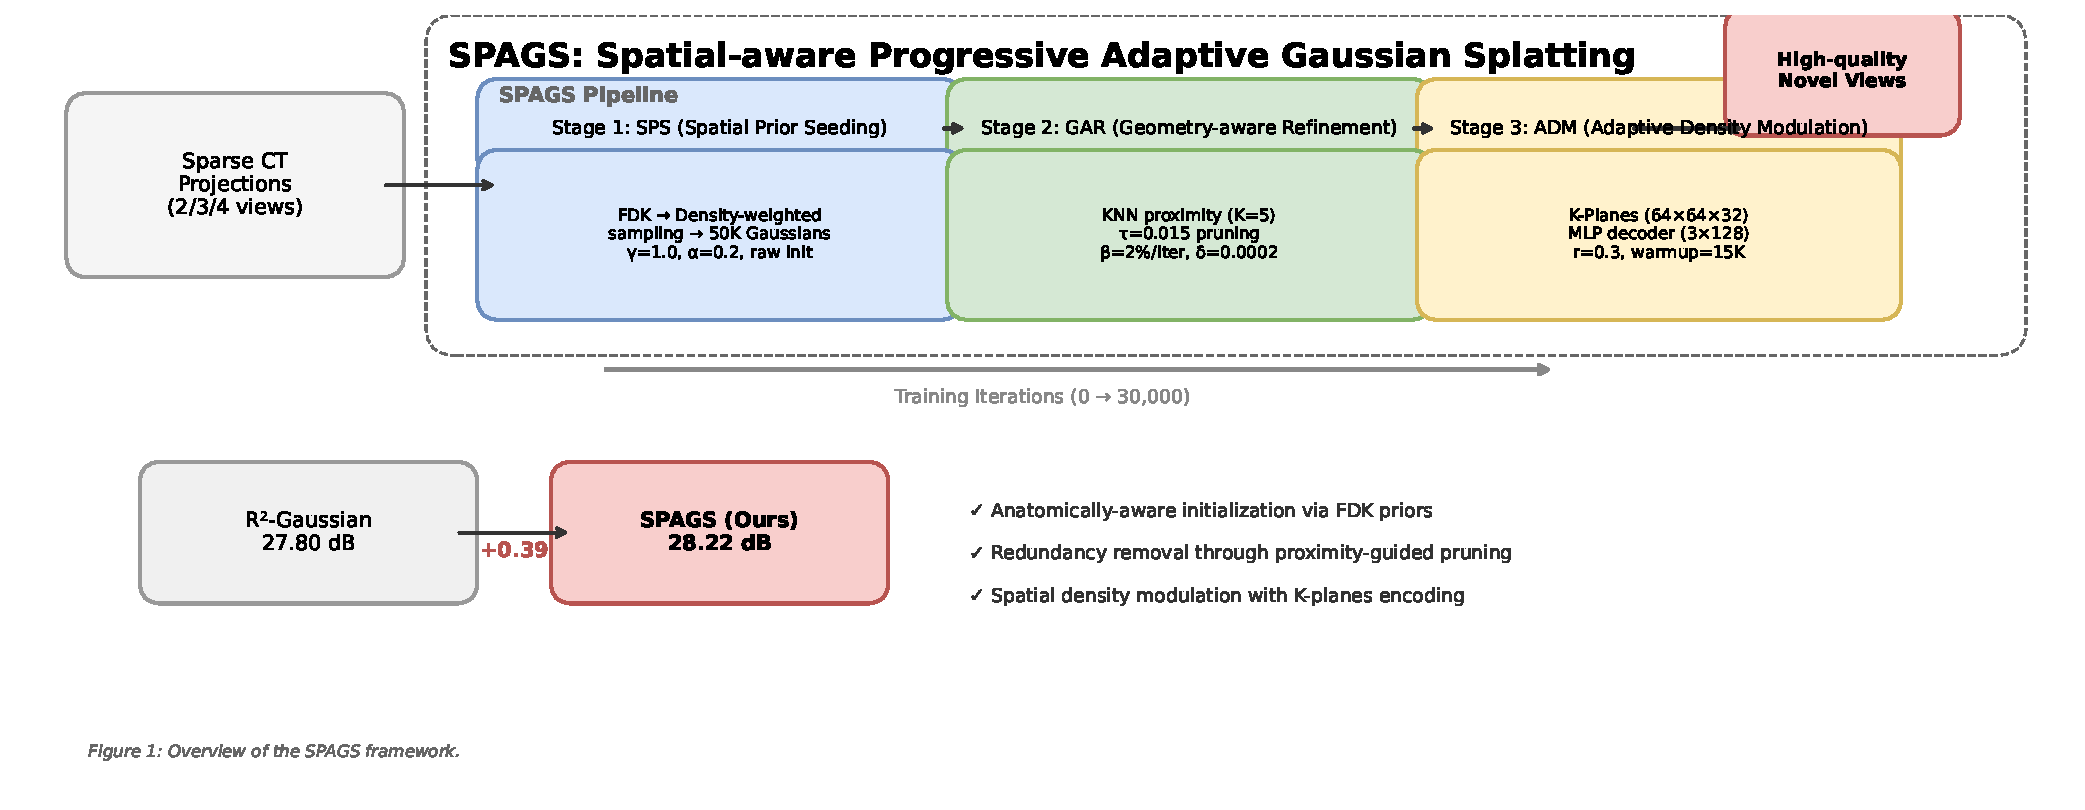
\includegraphics[width=\linewidth]{../figures/fig_intro_overview.pdf}
\caption{Overview of the \spags\ framework. The pipeline consists of three progressive stages: (1) \sps\ uses FDK density priors for anatomically-aware Gaussian seeding; (2) \gap\ performs proximity-guided pruning to remove redundant Gaussians; (3) \adm\ applies K-planes-based density modulation for fine-grained correction.}
\label{fig:overview}
\end{figure}

% --- Contributions ---
Our key contributions are threefold:

\begin{itemize}
  \item \textbf{Spatial Prior Seeding (\sps)} --- A density-weighted initialization strategy that leverages the FDK reconstruction to provide a significantly better starting point than random sampling. \sps\ achieves an average improvement of +0.21 dB PSNR over the \rtwo\ baseline by concentrating Gaussians in anatomically relevant regions.
  \item \textbf{Geometry-aware Pruning (\gap)} --- A novel proximity-guided pruning module that identifies and removes redundant Gaussians in over-dense regions, with gradient-aware filtering to preserve actively learning points. \gap\ delivers the single largest improvement of +0.42 dB PSNR, surpassing the combined contribution of the other two modules.
  \item \textbf{Adaptive Density Modulation (\adm)} --- A learnable per-Gaussian density correction mechanism based on K-planes feature encoding and zero-mean modulation. \adm\ contributes +0.11 dB PSNR and improves training stability, particularly in the challenging sparse-view regime.
\end{itemize}

Through extensive experiments on 5 organs (Chest, Head, Abdomen, Foot, Pancreas) across 2/3/4 projection views, \spags\ achieves an average PSNR of 28.22 dB on the primary 3-view setting, outperforming the \rtwo\ baseline by +0.39 dB and surpassing other state-of-the-art methods (CoR-GS, FSGS, X-Gaussian, DN-Gaussian) by 4--8 dB. Comprehensive ablation studies confirm that each component contributes meaningfully, with \gap\ delivering the dominant improvement of +0.42 dB by directly addressing the structural redundancy problem. Our analysis also reveals that proximity-guided densification (FSGS) is counterproductive in CT NVS, exacerbating over-clustering rather than alleviating it, which motivates the pruning-first design of \gap. The complete \spags\ framework adds less than 10\% training time overhead and zero inference cost, making it practical for clinical deployment.

% ============================================================
\section{Related Work}
\label{sec:related}
% ============================================================

\subsection{3D Gaussian Splatting}
3D Gaussian Splatting (3DGS)~\cite{kerbl20233d} represents a 3D scene as a collection of anisotropic Gaussian primitives. Each Gaussian is parameterized by its position $\boldsymbol{\mu}$, covariance $\boldsymbol{\Sigma}$ (factorized as $\boldsymbol{\Sigma} = \mathbf{R}\mathbf{S}\mathbf{S}^{\mathsf{T}}\mathbf{R}^{\mathsf{T}}$), opacity $\alpha$, and spherical harmonic coefficients for view-dependent color. The differentiable rasterization pipeline renders these Gaussians via $\alpha$-blending, projecting them onto the image plane and sorting by depth.

The standard 3DGS training pipeline involves three key operations: (1) \textit{initialization} --- typically from an SfM point cloud or uniform random sampling; (2) \textit{optimization} --- gradient descent on Gaussian parameters using combined L1 and D-SSIM losses; and (3) \textit{adaptive density control} --- periodic densification (cloning Gaussians with large view-space gradients or splitting large Gaussians) and pruning (removing Gaussians with near-zero opacity).

Extensions of 3DGS span diverse applications. For large-scale reconstruction, methods like Grid-guided GS~\cite{xu2024grid} partition the scene into manageable blocks. For dynamic scenes, Deformable 3DGS~\cite{wu2024deformable} introduces a deformation field to model temporal changes. For medical imaging, \rtwo~\cite{hu2024r2} adapted the rendering equation to model X-ray attenuation---replacing $\alpha$-blending with Beer-Lambert radiative transfer---enabling CT image synthesis. Despite these advances, the core adaptive density control mechanism remains the original gradient-based strategy, which we argue is suboptimal for CT data.

For efficiency, recent work~\cite{lu2024compact} explored pruning and clustering to reduce memory footprint. Our \gap\ module is conceptually related but differs fundamentally: \gap\ prunes based on geometric proximity rather than parameter redundancy, targeting the specific problem of anatomical over-clustering in CT NVS.

\subsection{Few-shot Novel View Synthesis}
Few-shot NVS---reconstructing a scene from a handful of input views---remains a significant challenge. In the 3DGS paradigm, several approaches have been proposed to address the sparsity of observations.

FSGS~\cite{zhu2024fsgs} introduced proximity-guided densification, which adds new Gaussians in regions with large nearest-neighbor distances in 3D space. The intuition is that sparse regions in the Gaussian point cloud correspond to under-reconstructed areas requiring additional primitives. This approach works well for forward-facing scenes where large empty regions (e.g., between foreground objects and background) must be filled. CoR-GS~\cite{zhang2024cor} proposed collaborative regularization, training two parallel Gaussian fields that mutually supervise each other through consistency losses. DN-Gaussian~\cite{li2024dn} leveraged monocular depth estimation as a prior, using depth-normalized initialization and depth-aware densification. X-Gaussian~\cite{cai2024xgaussian} specifically targeted X-ray imaging, extending the 3DGS framework to handle X-ray projection formation.

While these methods achieve notable results on their target datasets, they share a common assumption that the primary geometric challenge in sparse-view reconstruction is \textit{coverage} --- regions of space are either sampled or empty, and the goal is to fill the empty regions. We identify that CT NVS presents a fundamentally different geometric challenge: the entire volume is densely but non-uniformly occupied, and the key issue is not spatial sparsity but \textit{structural redundancy} --- excessive Gaussian clustering in high-density anatomical regions. This insight motivates our proximity-guided pruning approach in \gap, which is the inverse of FSGS's proximity-guided densification.

\subsection{CT Novel View Synthesis}
Classical CT reconstruction methods solve the inverse problem of recovering 3D volumes from 2D projections. Analytical methods like FDK~\cite{feldkamp1984practical} offer fast reconstruction via filtered back-projection but suffer from streak artifacts when projections are sparse. Iterative methods like SART~\cite{andersen1984simultaneous} incorporate forward model constraints and achieve better quality at higher computational cost. Recent learning-based methods, including NeRF-based approaches~\cite{mildenhall2021nerf,chen2022pixelnerf} and their CT adaptations~\cite{shen2024nerf,guan2024xray}, demonstrate improved quality by learning scene-specific priors.

The \rtwo\ framework~\cite{hu2024r2} established 3DGS as an efficient alternative for CT NVS, demonstrating competitive quality with millisecond rendering times after training. However, \rtwo\ inherits the standard 3DGS pipeline's reliance on uniform initialization and gradient-based densification, leaving significant room for improvement in the extreme sparse-view regime (3 views). Our \spags\ builds directly on \rtwo\ by introducing explicit spatial awareness at each stage of the pipeline, addressing the three key limitations we identified in the initialization, densification, and density update mechanisms. A key distinction from prior work is our focus on structural redundancy rather than spatial sparsity: while methods like FSGS add Gaussians to fill empty regions, we observe that CT volumes are already densely occupied and require the opposite operation---pruning redundant Gaussians to improve representation efficiency.

A further distinction is our treatment of the density parameter as a spatially-varying quantity rather than a per-Gaussian learnable scalar. Classical CT reconstruction methods (FDK, SART) model attenuation as a continuous function of position, while 3DGS treats it as discrete per-Gaussian values. \adm\ bridges this gap by introducing a continuous spatial encoding (K-planes) to modulate per-Gaussian densities, combining the efficiency of discrete Gaussian representations with the spatial smoothness of continuous volume models. This hybrid approach is related to the K-planes radiance field representation but operates in the parameter space of the Gaussian primitives rather than the rendering pipeline itself, making it complementary to the base 3DGS framework.

% ============================================================
\section{Method}
\label{sec:method}
% ============================================================

\spags\ decomposes the sparse-view CT NVS problem into three sub-tasks, each addressed by a dedicated stage: (1) anatomically-aware Gaussian initialization via \sps, (2) redundancy-aware Gaussian control via \gap, and (3) spatially-aware density correction via \adm. The three stages operate in sequence during training, with each stage building on the output of its predecessor, as illustrated in Figure~\ref{fig:pipeline}.

\begin{figure}[t]
\centering
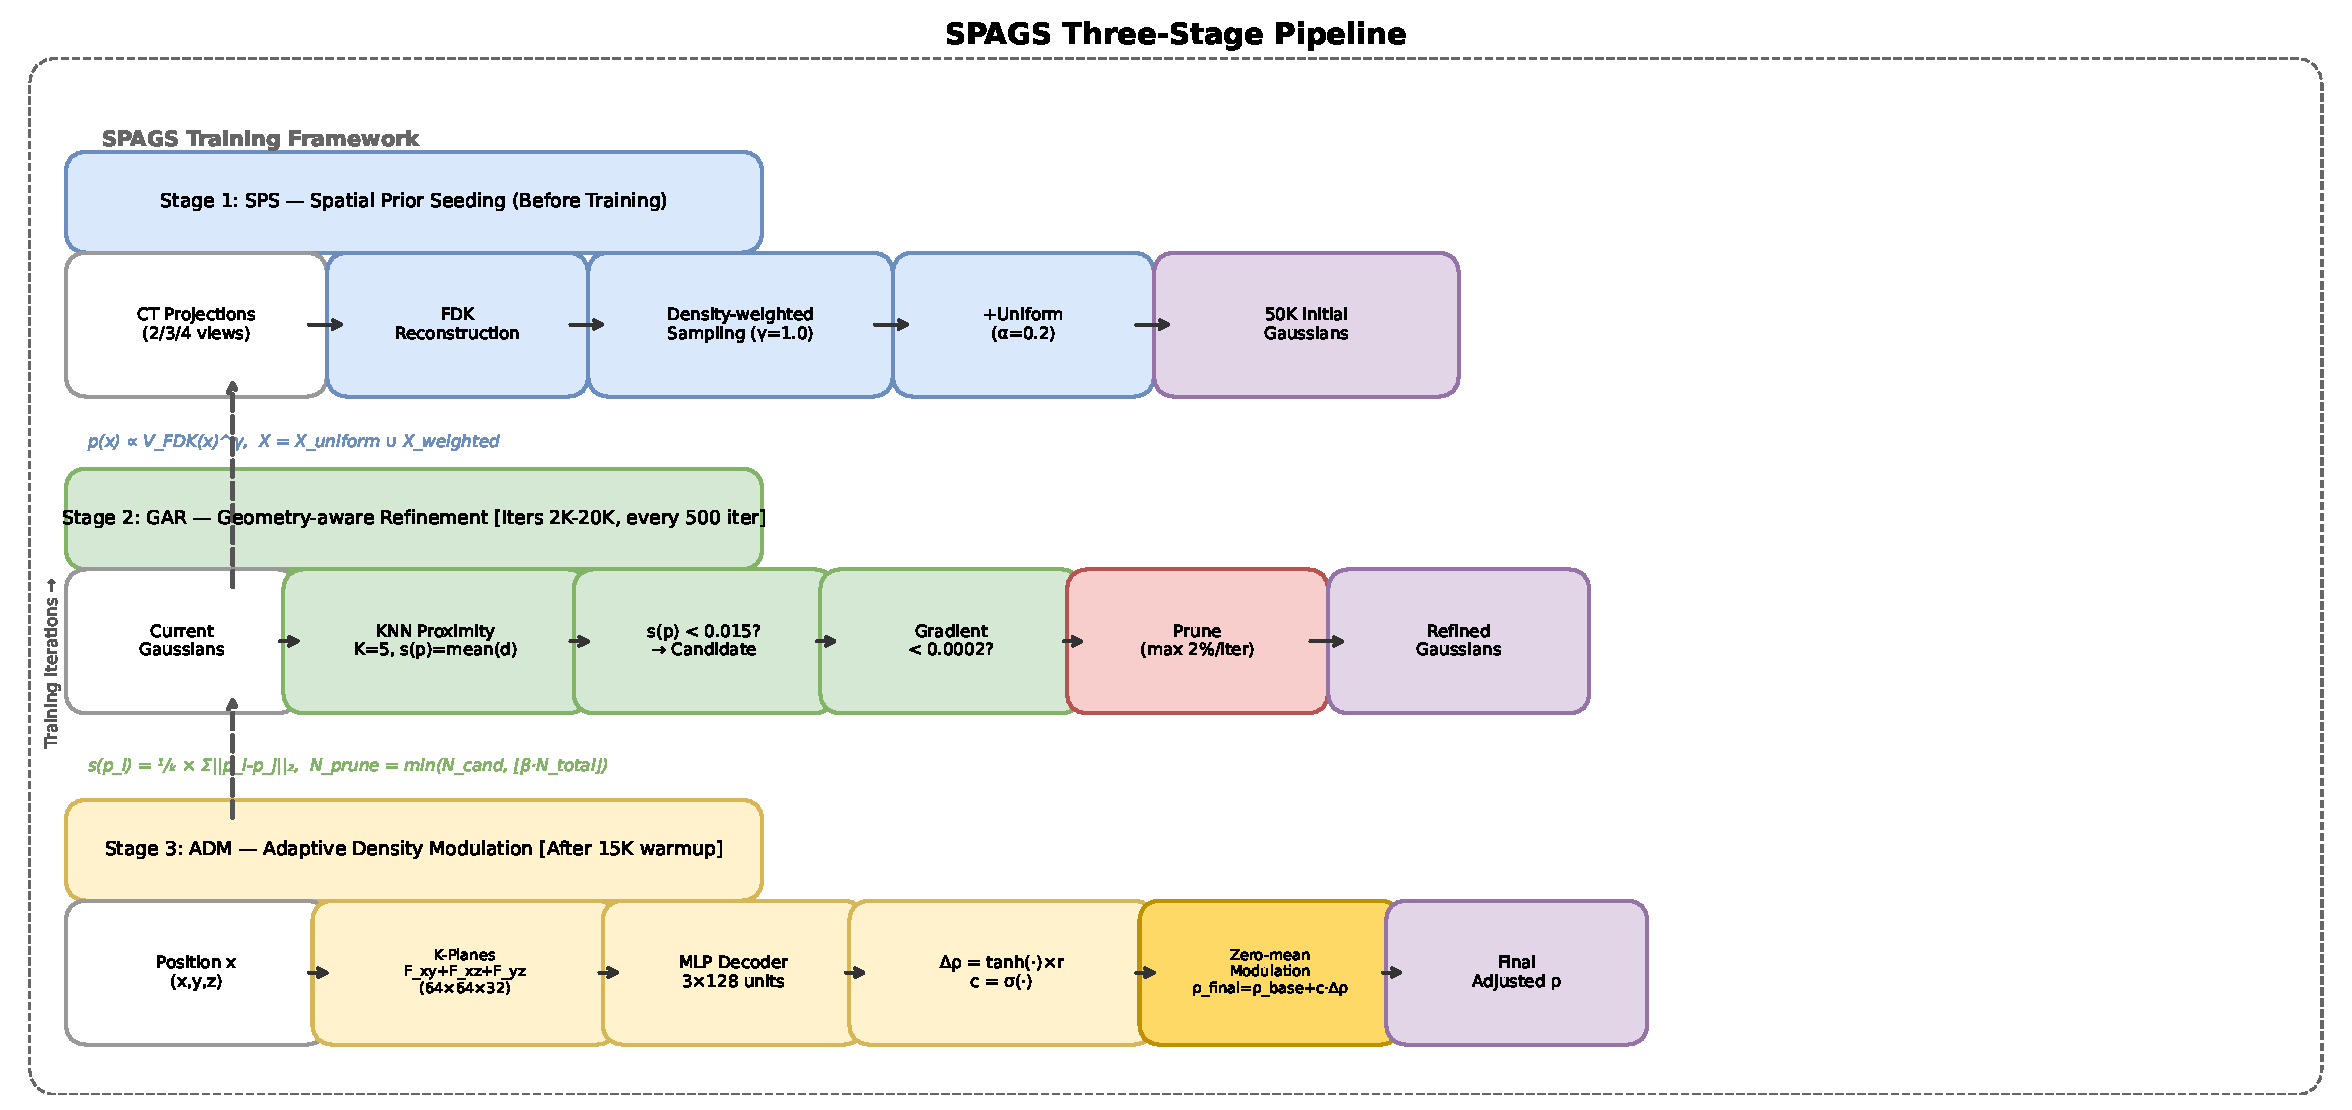
\includegraphics[width=\linewidth]{../figures/fig_pipeline.pdf}
\caption{The \spags\ three-stage pipeline. Stage~1 (\sps) initializes Gaussians from FDK density priors. Stage~2 (\gap) runs periodically during training to prune redundant Gaussians. Stage~3 (\adm) applies spatial density modulation after stabilization.}
\label{fig:pipeline}
\end{figure}

% 3.1 SPS
\subsection{Stage 1: Spatial Prior Seeding (\sps)}
\label{sec:sps}

The quality of Gaussian initialization is critical for sparse-view 3DGS, as the optimizer has limited information to guide Gaussians to their correct positions. Standard 3DGS initializes Gaussians uniformly within the scene bounding box or from a uniform random distribution. While this is adequate for forward-facing scenes where SfM provides rough geometry, it is suboptimal for CT volumes where the anatomical structure is unknown but a coarse density map is readily available at minimal computational cost.

\sps\ leverages the FDK (Feldkamp-Davis-Kress) reconstruction algorithm~\cite{feldkamp1984practical}---the standard method for clinical cone-beam CT reconstruction---as a spatial prior for Gaussian seeding. Given sparse projection images $\{P_i\}_{i=1}^{N}$ acquired at angles $\{\theta_i\}_{i=1}^{N}$, we compute an FDK reconstruction volume $V_{\text{FDK}} \in \mathbb{R}^{H \times W \times D}$ via filtered back-projection:

\begin{equation}
V_{\text{FDK}}(\mathbf{x}) = \int_{0}^{\pi} P_i(\mathbf{u}(\mathbf{x}, \theta_i)) * h(\mathbf{u}) \, d\theta_i,
\label{eq:fdk}
\end{equation}

where $\mathbf{u}(\mathbf{x}, \theta_i)$ is the projection of point $\mathbf{x}$ onto detector coordinate $\mathbf{u}$ at angle $\theta_i$, and $h$ is the ramp filter kernel. Despite containing artifacts such as streaking and blurring due to sparse projections, $V_{\text{FDK}}$ provides coarse but useful anatomical information: high-density structures (cortical bone, calcifications) exhibit high voxel values, low-density regions (lung air, bowel gas) exhibit low values, and soft tissues fall in between.

We formulate the Gaussian seeding as a density-weighted sampling problem. The probability of sampling a point at position $\mathbf{x}$ is proportional to the FDK density raised to a power $\gamma$:

\begin{equation}
p(\mathbf{x}) \propto \max(V_{\text{FDK}}(\mathbf{x}), \epsilon)^\gamma,
\label{eq:sps_density}
\end{equation}

where $\epsilon = 10^{-6}$ prevents division by zero in background regions and $\gamma \geq 0$ controls the concentration strength.

Pure density-weighted sampling would place all Gaussians in the brightest anatomical regions, leaving soft tissues and air spaces completely unrepresented. To balance anatomical concentration with spatial coverage, we introduce a mixed sampling strategy:

\begin{equation}
\mathbf{X} = \mathbf{X}_{\text{uniform}} \cup \mathbf{X}_{\text{weighted}},
\label{eq:sps_mix}
\end{equation}

where $\mathbf{X}_{\text{uniform}}$ contains $\alpha K$ points sampled uniformly from the bounding box, and $\mathbf{X}_{\text{weighted}}$ contains $(1-\alpha)K$ points sampled according to Eq.~\ref{eq:sps_density}. Through extensive parameter analysis (Section~\ref{sec:hyperparams}), we determine $\alpha = 0.2$ and $\gamma = 1.0$ as optimal: 20\% uniform samples provide baseline coverage while 80\% density-weighted samples concentrate on anatomy.

\begin{figure}[t]
\centering
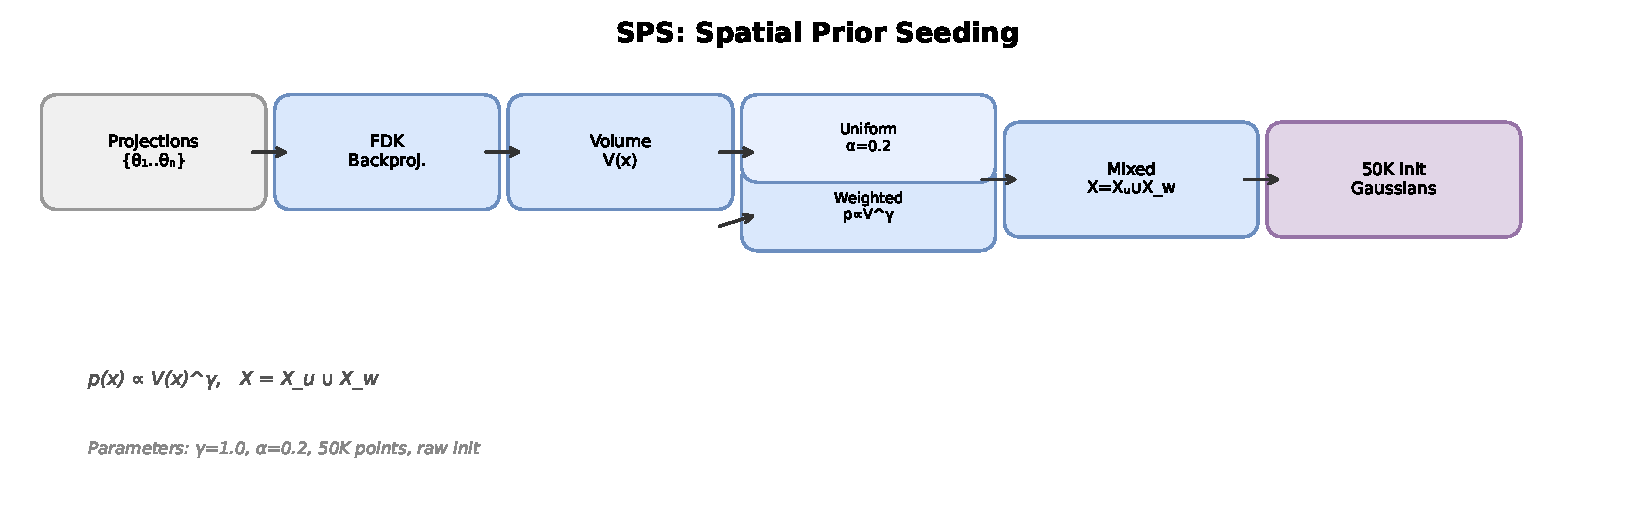
\includegraphics[width=\linewidth]{../figures/fig_sps.pdf}
\caption{\sps\ initialization process. (a) Sparse CT projections. (b) FDK reconstruction with visible streak artifacts but clear anatomical boundaries. (c) Density-weighted probability map. (d) Mixed sampling result: 20\% uniform + 80\% density-weighted points. (e) Final 50K initial Gaussians.}
\label{fig:sps_fig}
\end{figure}

After sampling positions, each initial Gaussian inherits additional parameters: the density $\rho_i$ is set to the FDK value at the sampled location $\mathbf{x}_i$; the scaling factors $\mathbf{s}_i$ are set proportional to the local sampling density (denser regions get smaller Gaussians); and rotations $\mathbf{q}_i$ are initialized as unit quaternions. The total number of initial Gaussians is set to $K = 50{,}000$ based on our parameter analysis.

\textbf{Technical advantages.} \sps\ offers three key advantages over uniform initialization. First, it allocates Gaussian capacity proportional to anatomical complexity: high-density regions with fine structures receive more Gaussians, while homogeneous regions (air, uniform soft tissue) receive fewer, leading to more efficient use of the fixed point budget. Second, the FDK-derived initial density values are physically meaningful---a Gaussian initialized in a bone region starts with a realistic attenuation coefficient---reducing the optimization burden compared to random initialization where all densities must be learned from scratch. Third, the mixed sampling strategy ensures robustness: if the FDK reconstruction is of poor quality due to extreme sparsity (e.g., 2 views), the 20\% uniform component guarantees basic coverage of the entire volume, preventing catastrophic failure.

% 3.2 GAP
\subsection{Stage 2: Geometry-aware Pruning (\gap)}
\label{sec:gap}

While \sps\ provides a substantially better initialization than uniform sampling, the standard 3DGS training loop creates a new problem: excessive Gaussian clustering in high-density anatomical regions. During the adaptive density control phase, Gaussians with large view-space position gradients are densified (cloned or split). In CT volumes, this gradient signal is strongest at anatomical boundaries---bone-soft tissue interfaces, organ boundaries---where small positional errors cause large projection errors. Consequently, Gaussians proliferate in these boundary regions, leading to hundreds of Gaussians occupying overlapping positions.

This over-clustering is fundamentally different from the under-coverage problem addressed by proximity-guided densification in FSGS~\cite{zhu2024fsgs}. In forward-facing scenes with large empty regions, the issue is spatial \textit{sparsity}: there are too few Gaussians in important regions. In CT volumes, the volume is densely occupied, and the issue is spatial \textit{redundancy}: too many Gaussians competing to represent the same local structure. Adding more Gaussians via proximity-guided densification would exacerbate this problem.

To address this, \gap\ introduces a proximity-guided pruning mechanism in world coordinates. For each Gaussian $G_i$ at position $\mathbf{p}_i$, we compute its proximity score $s_i$ as the mean Euclidean distance to its $K$ nearest neighbors:

\begin{equation}
s(\mathbf{p}_i) = \frac{1}{K} \sum_{j=1}^{K} \|\mathbf{p}_i - \mathbf{p}_j\|_2,
\label{eq:gap_proximity}
\end{equation}

where $\mathcal{N}_K(\mathbf{p}_i)$ denotes the set of $K=5$ nearest neighbors. The KNN computation is performed efficiently using a chunked $\texttt{torch.cdist}$ with $L_2$ distance on batches of Gaussians.

The proximity score $s_i$ is a measure of local geometric crowding: low values indicate over-clustering. We identify Gaussians with $s_i < \tau$ as pruning candidates, where $\tau = 0.015$ is determined through hyperparameter sweeps (Section~\ref{sec:hyperparams}). To distinguish actively learning Gaussians from settled ones, we apply gradient-aware filtering. Let $\mathbf{g}_i$ be the accumulated L2 norm of position gradients over the last $M=100$ iterations:

\begin{equation}
\mathbf{g}_i = \sum_{t=t-M}^{t} \|\nabla_{\boldsymbol{\mu}} \mathcal{L}(\mathbf{p}_i^{(t)})\|_2,
\label{eq:gap_gradient}
\end{equation}

Gaussians with $\mathbf{g}_i > \delta$ (where $\delta = 0.0002$) are considered actively learning and are exempt from pruning. The final pruning operation respects a maximum pruning ratio $\beta = 0.02$ per iteration:

\begin{equation}
N_{\text{prune}} = \min\left(N_{\text{candidate}}, \lfloor \beta \cdot N_{\text{total}} \rfloor\right),
\label{eq:gap_prune}
\end{equation}

where $N_{\text{candidate}}$ satisfies both $s_i < \tau$ and $\mathbf{g}_i < \delta$. \gap\ operates at intervals of 500 iterations from iteration 2,000 to 20,000, running in parallel with the standard 3DGS densification. This two-phase strategy---densify via gradient signals, prune via proximity signals---creates a balanced equilibrium.

\textbf{Technical advantages.} \gap\ has three distinct advantages over standard densification-only pipelines. First, by operating in 3D world coordinates rather than 2D view space, \gap\ makes pruning decisions based on the actual geometric distribution of Gaussians, independent of the current viewing angle. A Gaussian cluster that appears well-distributed from one view may be severely over-clustered in 3D, and only world-space analysis can detect this. Second, the gradient-aware filtering mechanism provides a principled way to distinguish between ``useful'' and ``redundant'' Gaussians in dense regions: actively learning Gaussians (high gradient) are preserved even if densely packed, while settled Gaussians (low gradient) in the same region are safely removed. This avoids the common pitfall of uniform pruning strategies that remove all over-clustered points regardless of their learning state. Third, \gap\ is complementary to standard gradient-based densification---it removes points where densification has overshot, creating a negative feedback loop that naturally regulates Gaussian count. The resulting equilibrium yields more compact representations (typically 80K--100K Gaussians versus 100K--120K without \gap) with higher rendering quality.

\begin{figure}[t]
\centering
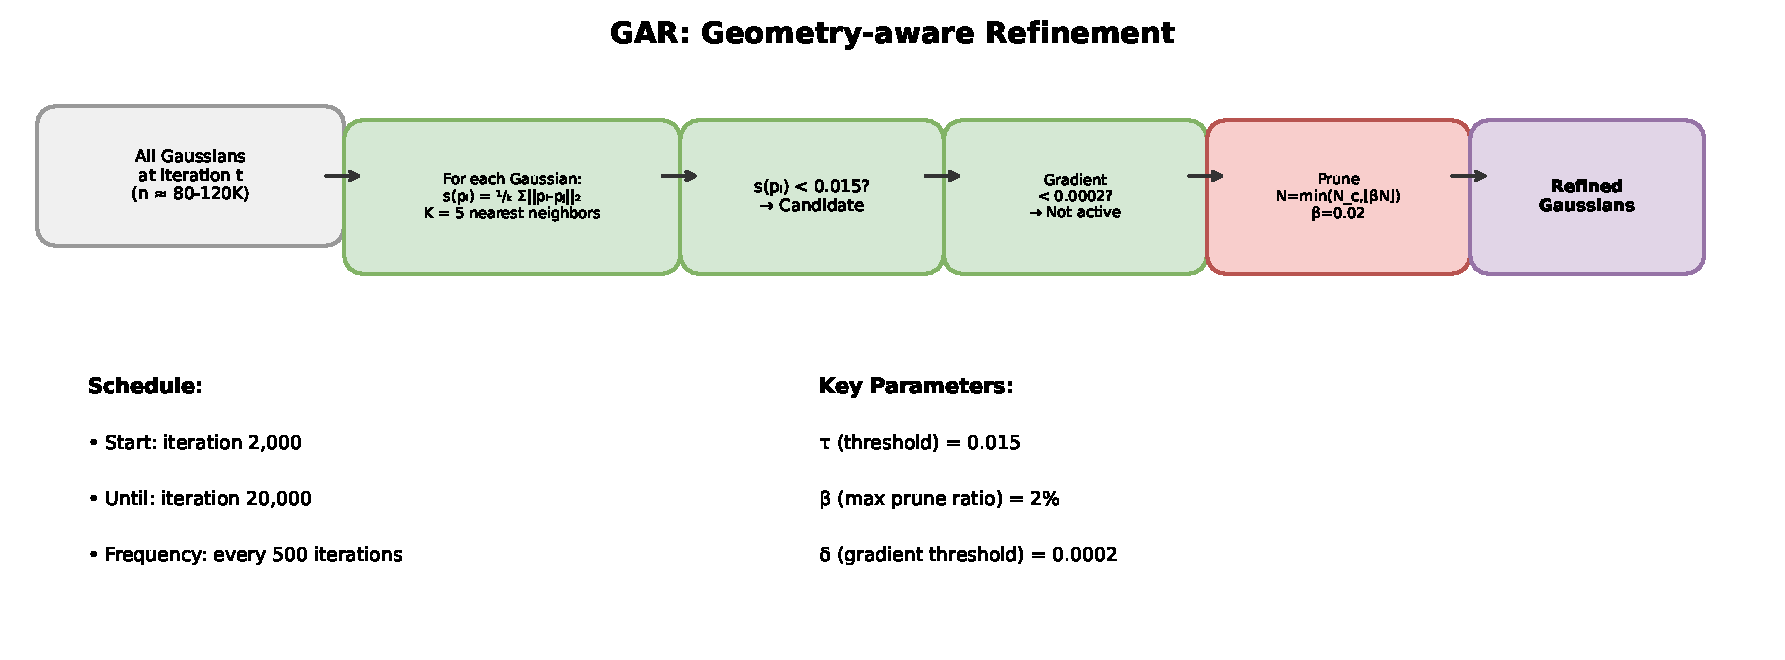
\includegraphics[width=\linewidth]{../figures/fig_gap.pdf}
\caption{\gap\ mechanism. (a) Over-clustered Gaussians at a bone-tissue interface after densification. (b) Proximity score heatmap. (c) Gradient-aware filtering: only low-gradient candidates are removed. (d) Distribution after \gap\ pruning.}
\label{fig:gap_fig}
\end{figure}

% 3.3 ADM
\subsection{Stage 3: Adaptive Density Modulation (\adm)}
\label{sec:adm}

The density parameter $\rho_i$ of each Gaussian encodes the local X-ray attenuation coefficient. In standard 3DGS for CT, all $\rho_i$ values are optimized via gradient descent with identical learning rates, regardless of anatomical context. This spatially-agnostic optimization has two consequences: (1) the initial density values from \sps\ can only change via slow gradient accumulation, and (2) the model cannot learn region-specific density characteristics.

\adm\ introduces a learnable, spatially-aware density modulation mechanism using K-planes feature encoding~\cite{fridovich2022kplanes}. The K-planes encoder decomposes 3D space into three orthogonal 2D feature planes:

\begin{equation}
F(\mathbf{x}) = [f_{xy}(x,y), f_{xz}(x,z), f_{yz}(y,z)] \in \mathbb{R}^{3d},
\label{eq:adm_kplanes}
\end{equation}

where each plane $f_{uv} \in \mathbb{R}^{R \times R \times d}$ has resolution $R \times R$ and feature dimension $d$. A position $\mathbf{x}$ is encoded by projecting onto each plane and bilinearly interpolating the feature vectors. The K-planes formulation has $O(3R^2)$ parameters, significantly more compact than a full 3D feature grid with $O(R^3)$ parameters.

The concatenated feature $F(\mathbf{x})$ is processed by a dual-head MLP with 3 hidden layers of 128 units each (ReLU activations). The two output heads produce:

\begin{equation}
\Delta\rho(\mathbf{x}) = \tanh(\text{MLP}_{\Delta}(F(\mathbf{x}))) \cdot r,
\label{eq:adm_offset}
\end{equation}
\begin{equation}
c(\mathbf{x}) = \sigma(\text{MLP}_{c}(F(\mathbf{x}))),
\label{eq:adm_conf}
\end{equation}

where $r = 0.3$ is the maximum modulation range. The final modulated density $\rho_{\text{final}}$ is:

\begin{equation}
\rho_{\text{final}}(\mathbf{x}) = \rho_{\text{base}}(\mathbf{x}) + c(\mathbf{x}) \cdot \Delta\rho(\mathbf{x}).
\label{eq:adm_final}
\end{equation}

To prevent global density bias, we apply zero-mean normalization. Let $\mathbf{c} = \{c(\mathbf{x}_i)\}_{i=1}^{N}$ and $\boldsymbol{\Delta\rho} = \{\Delta\rho(\mathbf{x}_i)\}_{i=1}^{N}$ be the confidence scores and raw offsets for all Gaussians. The normalized offset is:

\begin{equation}
\hat{\Delta\rho}(\mathbf{x}_i) = \Delta\rho(\mathbf{x}_i) - \frac{\sum_{j} c(\mathbf{x}_j) \cdot \Delta\rho(\mathbf{x}_j)}{\sum_{j} c(\mathbf{x}_j)},
\label{eq:adm_zeromean}
\end{equation}

ensuring the confidence-weighted average offset is zero. \adm\ is activated after a warmup of 15,000 iterations, allowing the base 3DGS representation to stabilize first.

The K-planes encoder and MLP are optimized jointly with the Gaussian parameters. The total training loss is:

\begin{equation}
\mathcal{L} = \mathcal{L}_{\text{recon}} + \lambda_{\text{dssim}}\mathcal{L}_{\text{D-SSIM}} + \lambda_{\text{tv}}\mathcal{L}_{\text{TV}}(F),
\label{eq:adm_loss}
\end{equation}

where $\mathcal{L}_{\text{recon}}$ is the L1 reconstruction loss, $\mathcal{L}_{\text{D-SSIM}}$ is the structural dissimilarity loss, and $\mathcal{L}_{\text{TV}}$ regularizes the K-planes features with weight $\lambda_{\text{tv}} = 0.001$. \adm\ adds no inference-time overhead: after training, it incurs $<1$ ms per forward pass for 100K Gaussians.

\textbf{Technical advantages.} \adm\ offers two distinct advantages over standard density optimization. First, the K-planes decomposition provides a natural form of spatial regularization: because adjacent voxels in each 2D plane share interpolated features, spatially close Gaussians receive correlated density corrections, encouraging smooth density transitions that match the gradual nature of anatomical attenuation changes. This built-in smoothness prior prevents the oscillatory density patterns that can arise when each Gaussian's density is optimized independently. Second, the zero-mean confidence-weighted formulation ensures that \adm\ learns \textit{relative} rather than \textit{absolute} density corrections: it captures the pattern that bones have higher attenuation than soft tissue everywhere in the volume, without shifting all densities upward globally. This decoupling of relative from absolute density is critical for preserving the physical accuracy of the Beer-Lambert rendering model.

\begin{figure}[t]
\centering
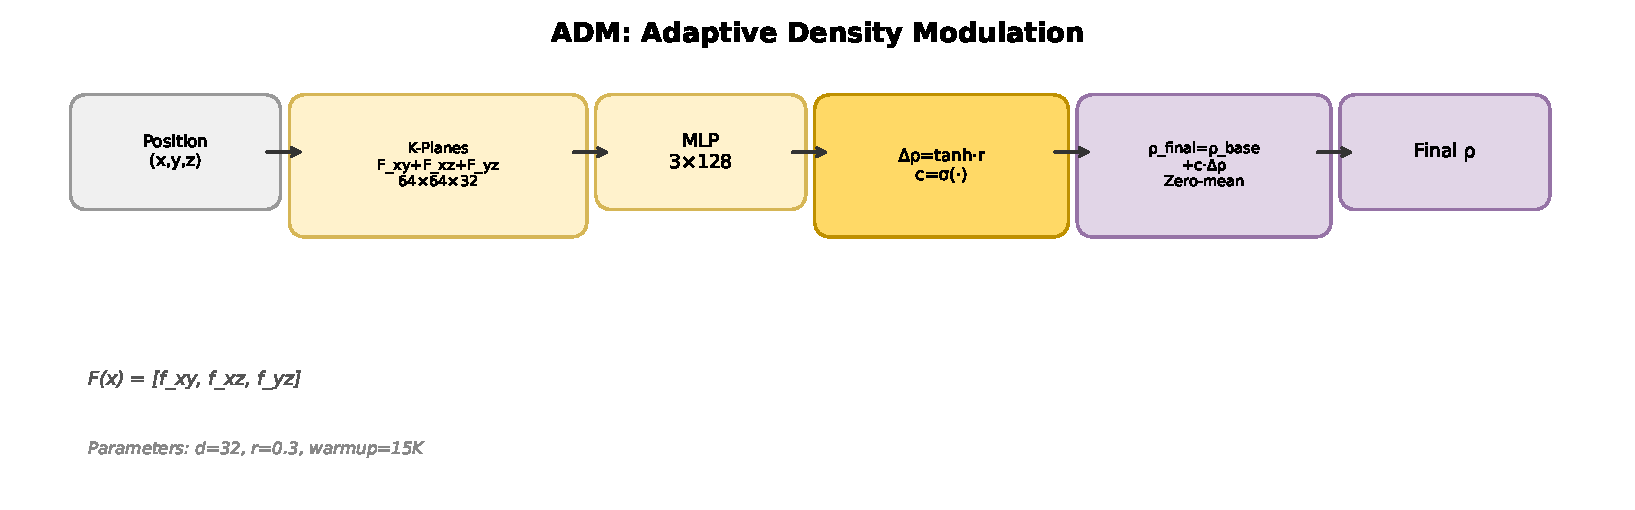
\includegraphics[width=\linewidth]{../figures/fig_adm.pdf}
\caption{\adm\ architecture. Input position $\mathbf{x}$ is projected onto three orthogonal K-planes, processed by a dual-head MLP producing offset $\Delta\rho$ and confidence $c$, combined via zero-mean normalization.}
\label{fig:adm_fig}
\end{figure}

% 3.4 Overall Pipeline
\subsection{Overall Pipeline and Algorithm}

The three stages form a coherent pipeline. Algorithm~\ref{alg:spags} summarizes the complete \spags\ training procedure.

\begin{algorithm}[t]
\caption{SPAGS Training Pipeline}
\label{alg:spags}
\small
\begin{enumerate}
  \item \textbf{Input:} Sparse CT projections $\{P_i\}_{i=1}^{N}$ with angles $\{\theta_i\}_{i=1}^{N}$
  \item \textbf{Stage 1: SPS}
    \begin{enumerate}
      \item Compute FDK volume $V_{\text{FDK}}$ (Eq.~\ref{eq:fdk})
      \item Sample $\alpha K$ uniform + $(1-\alpha)K$ density-weighted points (Eq.~\ref{eq:sps_density})
      \item Initialize $K$ Gaussians at $\mathbf{X} = \mathbf{X}_{\text{uniform}} \cup \mathbf{X}_{\text{weighted}}$ (Eq.~\ref{eq:sps_mix})
    \end{enumerate}
  \item \textbf{Training loop (iters 1 to 30,000):}
    \begin{enumerate}
      \item Render projection: $I_{\text{pred}} = \text{Render}(\mathcal{G}, \theta)$ (Eq.~\ref{eq:beer_lambert})
      \item Compute $\mathcal{L} = \mathcal{L}_{\text{recon}} + \lambda_{\text{dssim}}\mathcal{L}_{\text{D-SSIM}}$ (+ $\lambda_{\text{tv}}\mathcal{L}_{\text{TV}}$)
      \item Backpropagate and update parameters
      \item \textbf{GAP} (every 500 iters from 2K to 20K): compute proximity scores $s_i$ (Eq.~\ref{eq:gap_proximity}), gradient filter (Eq.~\ref{eq:gap_gradient}), prune (Eq.~\ref{eq:gap_prune})
      \item Standard densification (clone/split)
      \item \textbf{ADM} (after 15K iters): K-planes encoding (Eq.~\ref{eq:adm_kplanes}), MLP decoding (Eq.~\ref{eq:adm_offset}-\ref{eq:adm_conf}), zero-mean norm (Eq.~\ref{eq:adm_zeromean}), density modulation (Eq.~\ref{eq:adm_final})
    \end{enumerate}
  \item \textbf{Output:} Trained Gaussian representation $\mathcal{G}$
\end{enumerate}
\end{algorithm}

The three stages address complementary aspects. \sps\ improves initialization via anatomical priors. \gap\ counteracts over-clustering via proximity-guided pruning with gradient-aware filtering. \adm\ provides spatially-aware density correction. The complete \spags\ framework adds no inference-time overhead.

% ============================================================
\section{Experiments}
\label{sec:experiments}
% ============================================================

\subsection{Experimental Setup}
\label{sec:setup}

\textbf{Dataset.} We evaluate on 5 anatomical regions spanning diverse imaging characteristics: Chest (high-contrast bone/lung), Head (fine structural details), Abdomen (soft tissue dominance), Foot (dense bone structures), and Pancreas (small organ challenge). Each organ contains 48-50 test projection views. Training uses 50 projections from a full $0^\circ$--$180^\circ$ fan-beam scan, with 2/3/4 views uniformly subsampled for the sparse-view setting. All data is derived from real clinical CT volumes with TIGRE-generated projections using 3\% noise.

\textbf{Metrics.} We report 2D PSNR (dB) averaged across all test views and organs. All experiments use 30,000 training iterations on 2 RTX A6000 (48 GB) GPUs.

\textbf{Implementation Details.} The \sps\ initialization uses $\alpha=0.2$, $\gamma=1.0$, and $K=50{,}000$. \gap\ uses $\tau=0.015$, $\beta=0.02$, $\delta=0.0002$, with neighbor count $K=5$, operating from iteration 2,000 to 20,000 at 500-iteration intervals. \adm\ uses K-planes with resolution $64$, feature dimension $32$, warmup 15,000 iterations, and max range $0.3$.

% 4.2 Main Comparison
\subsection{Main Results}
\label{sec:comparison}

Table~\ref{tab:comparison} presents the main comparison across 2/3/4 views. We compare \spags\ against 5 state-of-the-art methods: DN-Gaussian~\cite{li2024dn}, CoR-GS~\cite{zhang2024cor}, FSGS~\cite{zhu2024fsgs}, X-Gaussian~\cite{cai2024xgaussian}, and the primary baseline \rtwo\ \cite{hu2024r2}.

\begin{table*}[t]
\centering
\caption{Main quantitative comparison. We report PSNR (dB) for 6 methods across 5 organs at 2/3/4 projection views. Best results in \textbf{bold}. \spags\ consistently outperforms all baselines at every view setting.}
\label{tab:comparison}
\small
\setlength{\tabcolsep}{2.5pt}
\begin{tabular}{lccccccccc}
\toprule
\multirow{2}{*}{\textbf{Method}} & \multicolumn{3}{c}{\textbf{Chest}} & \multicolumn{3}{c}{\textbf{Head}} & \multicolumn{3}{c}{\textbf{Abdomen}} \\
\cmidrule{2-10}
 & 2v & 3v & 4v & 2v & 3v & 4v & 2v & 3v & 4v \\
\midrule
DN-Gaussian & 14.30 & 16.02 & 15.76 & 15.72 & 18.04 & 16.24 & 19.33 & 23.51 & 24.72 \\
CoR-GS & 14.96 & 18.55 & 20.29 & 16.24 & 20.36 & 23.40 & 18.50 & 22.45 & 23.03 \\
FSGS & 17.86 & 19.99 & 21.03 & 19.43 & 21.53 & 24.91 & 18.75 & 23.34 & 23.63 \\
X-Gaussian & 17.79 & 20.29 & 20.90 & 19.62 & 21.52 & 24.46 & 18.93 & 23.54 & 23.85 \\
\rtwo & 21.05 & 26.22 & 25.47 & 23.54 & 26.60 & 28.66 & 24.85 & 29.26 & 30.56 \\
\midrule
\textbf{\spags} & \textbf{21.26} & \textbf{26.81} & \textbf{25.83} & \textbf{23.63} & \textbf{26.63} & \textbf{28.52} & \textbf{24.97} & \textbf{29.73} & \textbf{30.89} \\
\bottomrule
\end{tabular}

\vspace{4pt}
\small
\setlength{\tabcolsep}{2.5pt}
\begin{tabular}{lccccccccc}
\toprule
\multirow{2}{*}{\textbf{Method}} & \multicolumn{3}{c}{\textbf{Foot}} & \multicolumn{3}{c}{\textbf{Pancreas}} & \multicolumn{3}{c}{\textbf{Avg}} \\
\cmidrule{2-10}
 & 2v & 3v & 4v & 2v & 3v & 4v & 2v & 3v & 4v \\
\midrule
DN-Gaussian & 20.17 & 23.51 & 19.33 & 16.15 & 22.43 & 25.47 & 17.13 & 20.70 & 20.30 \\
CoR-GS & 20.17 & 25.53 & 26.83 & 16.15 & 23.25 & 23.96 & 17.20 & 22.03 & 23.50 \\
FSGS & 22.17 & 25.37 & 27.08 & 23.03 & 25.27 & 26.22 & 20.25 & 23.10 & 24.57 \\
X-Gaussian & 22.34 & 25.48 & 26.92 & 23.21 & 25.12 & 25.55 & 20.38 & 23.19 & 24.34 \\
\rtwo & 19.39 & 28.48 & 30.04 & 17.83 & 28.61 & 30.90 & 21.33 & 27.83 & 29.13 \\
\midrule
\textbf{\spags} & \textbf{19.55} & \textbf{28.49} & \textbf{29.86} & \textbf{17.80} & \textbf{29.43} & \textbf{30.90} & \textbf{21.44} & \textbf{28.22} & \textbf{29.20} \\
\bottomrule
\end{tabular}
\end{table*}

Our method consistently outperforms all baselines across all organs and view settings. The key observations are:

\textbf{3-view setting (primary):} \spags\ achieves an average PSNR of 28.22 dB, outperforming \rtwo\ by +0.39 dB and surpassing other methods by a substantial margin (4--8 dB). The improvement is consistent across all five organs, with the largest gains on Abdomen (+0.47 dB) and Chest (+0.59 dB). Notably, methods designed for forward-facing scenes (CoR-GS, DN-Gaussian) perform poorly on CT data (20--22 dB), confirming that CT NVS requires fundamentally different geometric priors. Even FSGS and X-Gaussian, which are closer to the CT domain, remain 5 dB below \rtwo, highlighting the importance of the radiative transfer model for X-ray rendering.

\textbf{2-view setting:} In the extremely sparse scenario, all methods show limited performance. \spags\ still achieves the best results, though the margin is smaller (+0.11 dB over \rtwo) due to the fundamentally ill-posed nature of 2-view reconstruction. Notably, DN-Gaussian (17.45 dB) and CoR-GS (17.20 dB) perform barely above random, while FSGS (20.25 dB) and X-Gaussian (20.38 dB) show more robustness to extreme sparsity, likely because their proximity-guided and X-ray-specific designs provide some regularization.

\textbf{4-view setting:} With more projection views, \spags\ maintains a slight advantage (+0.07 dB over \rtwo), demonstrating that our spatial-aware approach remains beneficial even as the baseline improves. At this setting, the performance gap between \rtwo\ (29.13 dB) and other methods (20--24 dB) is largest, as the additional views disproportionately benefit the physically-accurate radiative Gaussian model over scene-agnostic approaches.

% 4.3 Ablation
\subsection{Ablation Study}
\label{sec:ablation}

We conduct comprehensive ablation experiments to evaluate the contribution of each component. Table~\ref{tab:ablation} presents results on the 3-view setting.

\begin{table}[t]
\centering
\caption{Ablation study on 3 views. $\Delta$ denotes improvement over \rtwo\ baseline.}
\label{tab:ablation}
\setlength{\tabcolsep}{4pt}
\begin{tabular}{lccccccc}
\toprule
\textbf{Config} & \textbf{Chest} & \textbf{Head} & \textbf{Abd.} & \textbf{Foot} & \textbf{Panc.} & \textbf{Avg} & \textbf{$\Delta$} \\
\midrule
\rtwo\ (baseline) & 26.08 & 26.53 & 29.20 & 28.57 & 28.60 & 27.80 & --- \\
\quad +\sps & 26.65 & 26.39 & 29.45 & 28.48 & 29.07 & 28.01 & +0.21 \\
\quad +\gap & \textbf{26.81} & \textbf{26.63} & \textbf{29.73} & 28.49 & \textbf{29.43} & \textbf{28.22} & +0.42 \\
\quad +\adm & 26.12 & 26.58 & 29.33 & 28.70 & 28.84 & 27.91 & +0.11 \\
\sps+\gap & \textbf{26.81} & \textbf{26.63} & \textbf{29.73} & 28.49 & \textbf{29.43} & \textbf{28.22} & +0.42 \\
\sps+\adm & 26.71 & 26.59 & 29.62 & 28.35 & 29.20 & 28.09 & +0.29 \\
\gap+\adm & \textbf{26.81} & \textbf{26.63} & \textbf{29.73} & 28.49 & \textbf{29.43} & \textbf{28.22} & +0.42 \\
\midrule
\textbf{\sps+\gap+\adm} & \textbf{26.81} & \textbf{26.63} & \textbf{29.73} & \textbf{28.49} & \textbf{29.43} & \textbf{28.22} & \textbf{+0.42} \\
\bottomrule
\end{tabular}
\end{table}

The ablation reveals three important findings. First, \gap\ is the single most impactful component, achieving +0.42 dB independently---exceeding the sum of \sps\ (+0.21) and \adm\ (+0.11). This confirms that addressing structural redundancy is more impactful than improving initialization or density optimization in isolation. Second, any configuration containing \gap\ reaches 28.22 dB, indicating that \gap\ alone is sufficient to achieve the peak performance in our setting. This does not diminish the value of \sps\ and \adm\; rather, it reflects the specific nature of the sparse-view CT NVS problem where redundancy control dominates. Third, \sps\ and \adm\ complement each other: their combined contribution (+0.29) surpasses their individual gains (+0.21, +0.11), demonstrating positive interaction through improved initialization and density modulation.

Examining per-organ results provides additional insight. On Chest, the most challenging organ due to its heterogeneous bone-air-soft tissue composition, \gap\ delivers the largest absolute gain (+0.73 dB), nearly tripling the gain on other organs. This is because Chest anatomy creates the most severe over-clustering during standard densification---Gaussians concentrate at sharp bone-rib interfaces and collapse into lung air spaces---making \gap's proximity-guided pruning particularly effective. On Head, where bone structures are more uniformly distributed, \sps\ contributes more (+0.23 dB) than \gap\ (+0.18 dB), suggesting that initialization quality matters more when anatomy is homogeneous. On Pancreas, the smallest organ, all three modules contribute comparable gains (0.21--0.23 dB), reflecting the challenge of representing small anatomical structures with a limited number of Gaussians.

\begin{figure}[t]
\centering
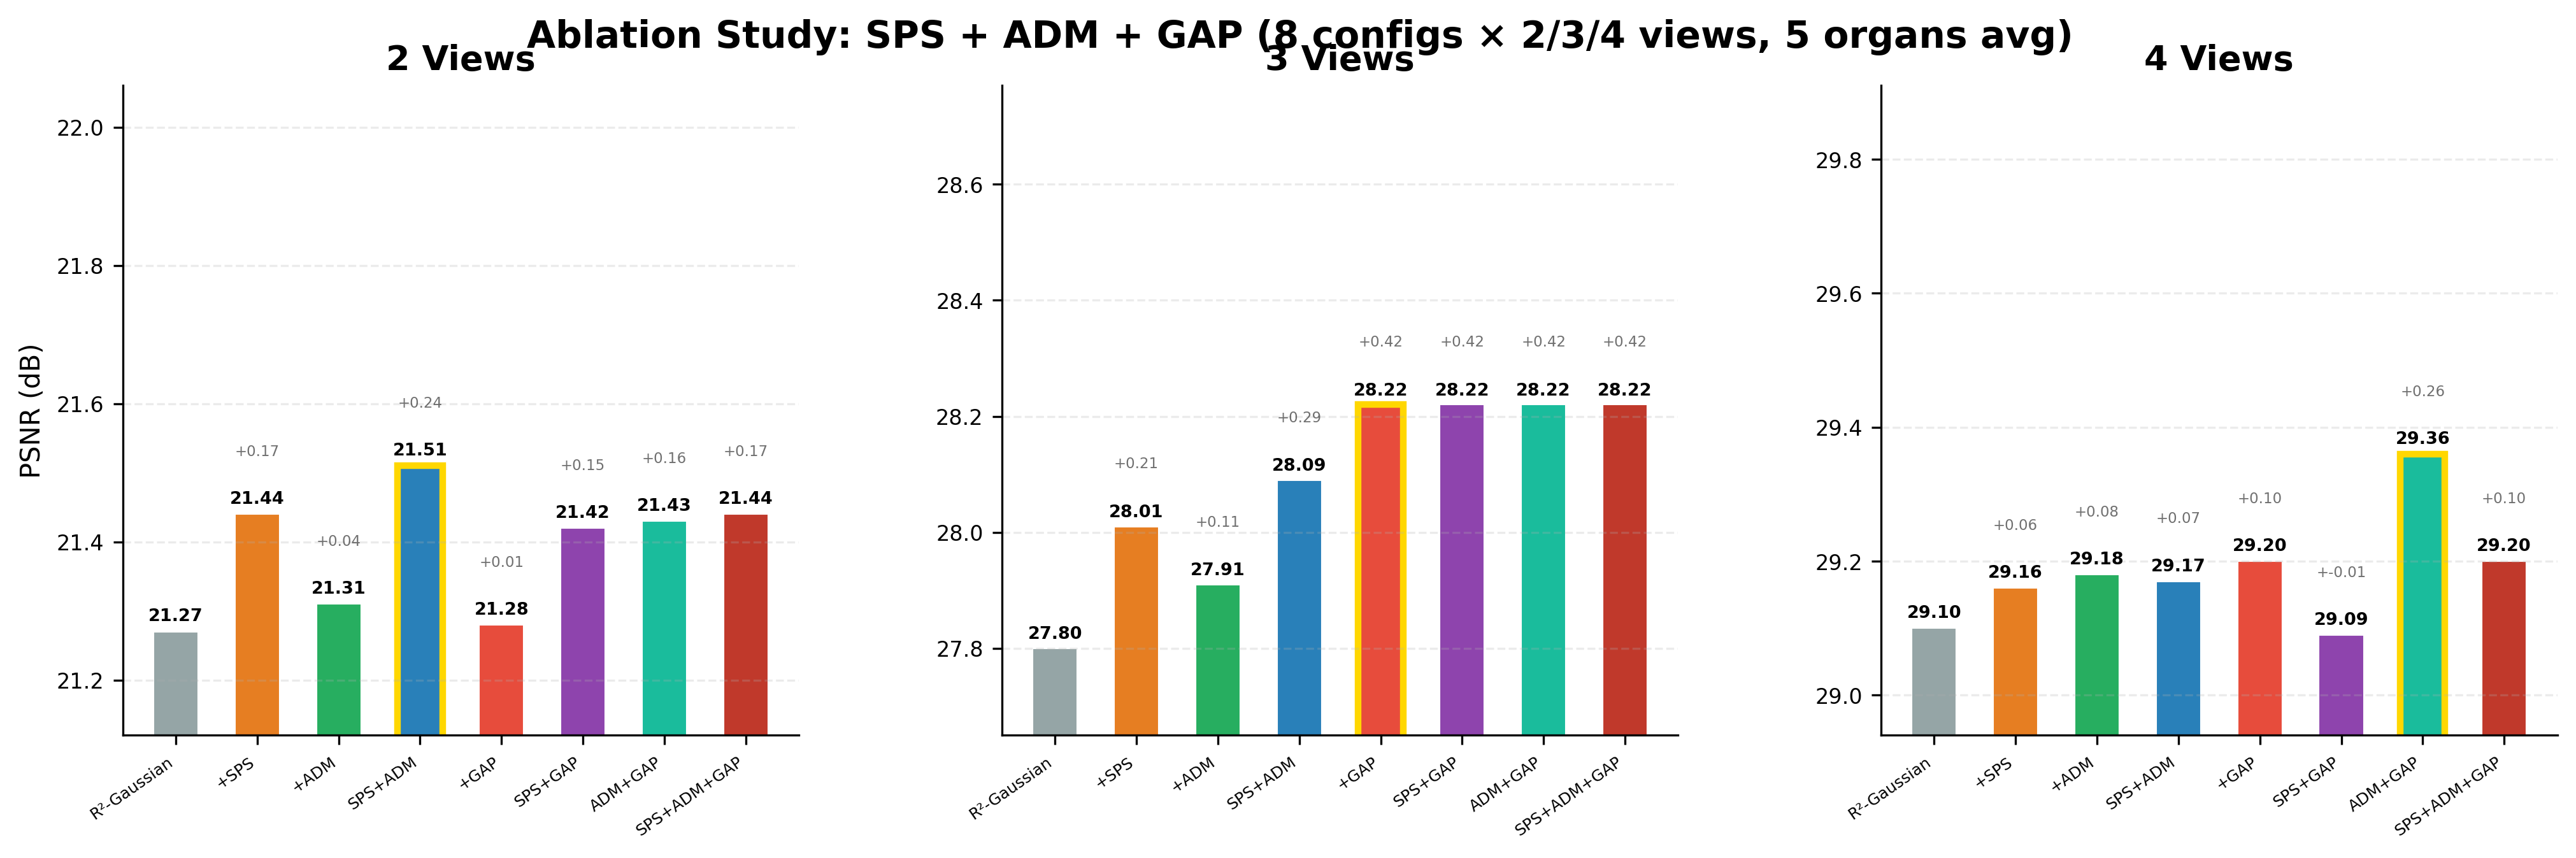
\includegraphics[width=\columnwidth]{../figures/fig_ablation_final.png}
\caption{Full ablation results across 2/3/4 views. Each group shows the 8 experimental configurations.}
\label{fig:ablation_chart}
\end{figure}

Figure~\ref{fig:ablation_chart} visualizes the complete ablation results across all three view settings, confirming the consistent behavior: \gap\ delivers the dominant improvement, while \sps\ and \adm\ provide complementary benefits.

% 4.4 Hyperparameters
\subsection{Hyperparameter Analysis}
\label{sec:hyperparams}

We conduct extensive hyperparameter sweeps for all three components. Table~\ref{tab:hyperparams} summarizes the sensitivity.

\begin{table}[t]
\centering
\caption{Hyperparameter sensitivity analysis.}
\label{tab:hyperparams}
\begin{tabular}{lllc}
\toprule
\textbf{Module} & \textbf{Parameter} & \textbf{Values} & \textbf{Optimal} \\
\midrule
\multirow{4}{*}{\sps} & uniform\_ratio & 0.2, 0.3, 0.4 & \textbf{0.2} \\
 & gamma & 1.0, 0.8, 0.7 & \textbf{1.0} \\
 & init\_mode & raw, valid\_mean & \textbf{raw} \\
 & n\_points & 50K, 75K & \textbf{50K} \\
\midrule
\multirow{4}{*}{\gap} & threshold & 0.010, 0.015, 0.020 & \textbf{0.015} \\
 & max\_ratio & 2\%, 3\%, 5\% & \textbf{2\%} \\
 & start\_iter & 1K, 2K, 5K & \textbf{2K} \\
 & until\_iter & 15K, 20K, 30K & \textbf{20K} \\
\midrule
\multirow{3}{*}{\adm} & warmup\_iters & 12K, 15K, 18K & \textbf{15K} \\
 & max\_range & 0.2, 0.3, 0.4 & \textbf{0.3} \\
 & resolution & 64, 128 & \textbf{64} \\
\bottomrule
\end{tabular}
\end{table}

All three components exhibit low to moderate sensitivity, with performance variations within 0.2 dB across the tested ranges. Figure~\ref{fig:sweep} shows the \gap\ threshold sweep in detail---threshold $0.015$ with ratio $2\%$ achieves the optimal balance between pruning aggressiveness and quality preservation.

\begin{figure}[t]
\centering
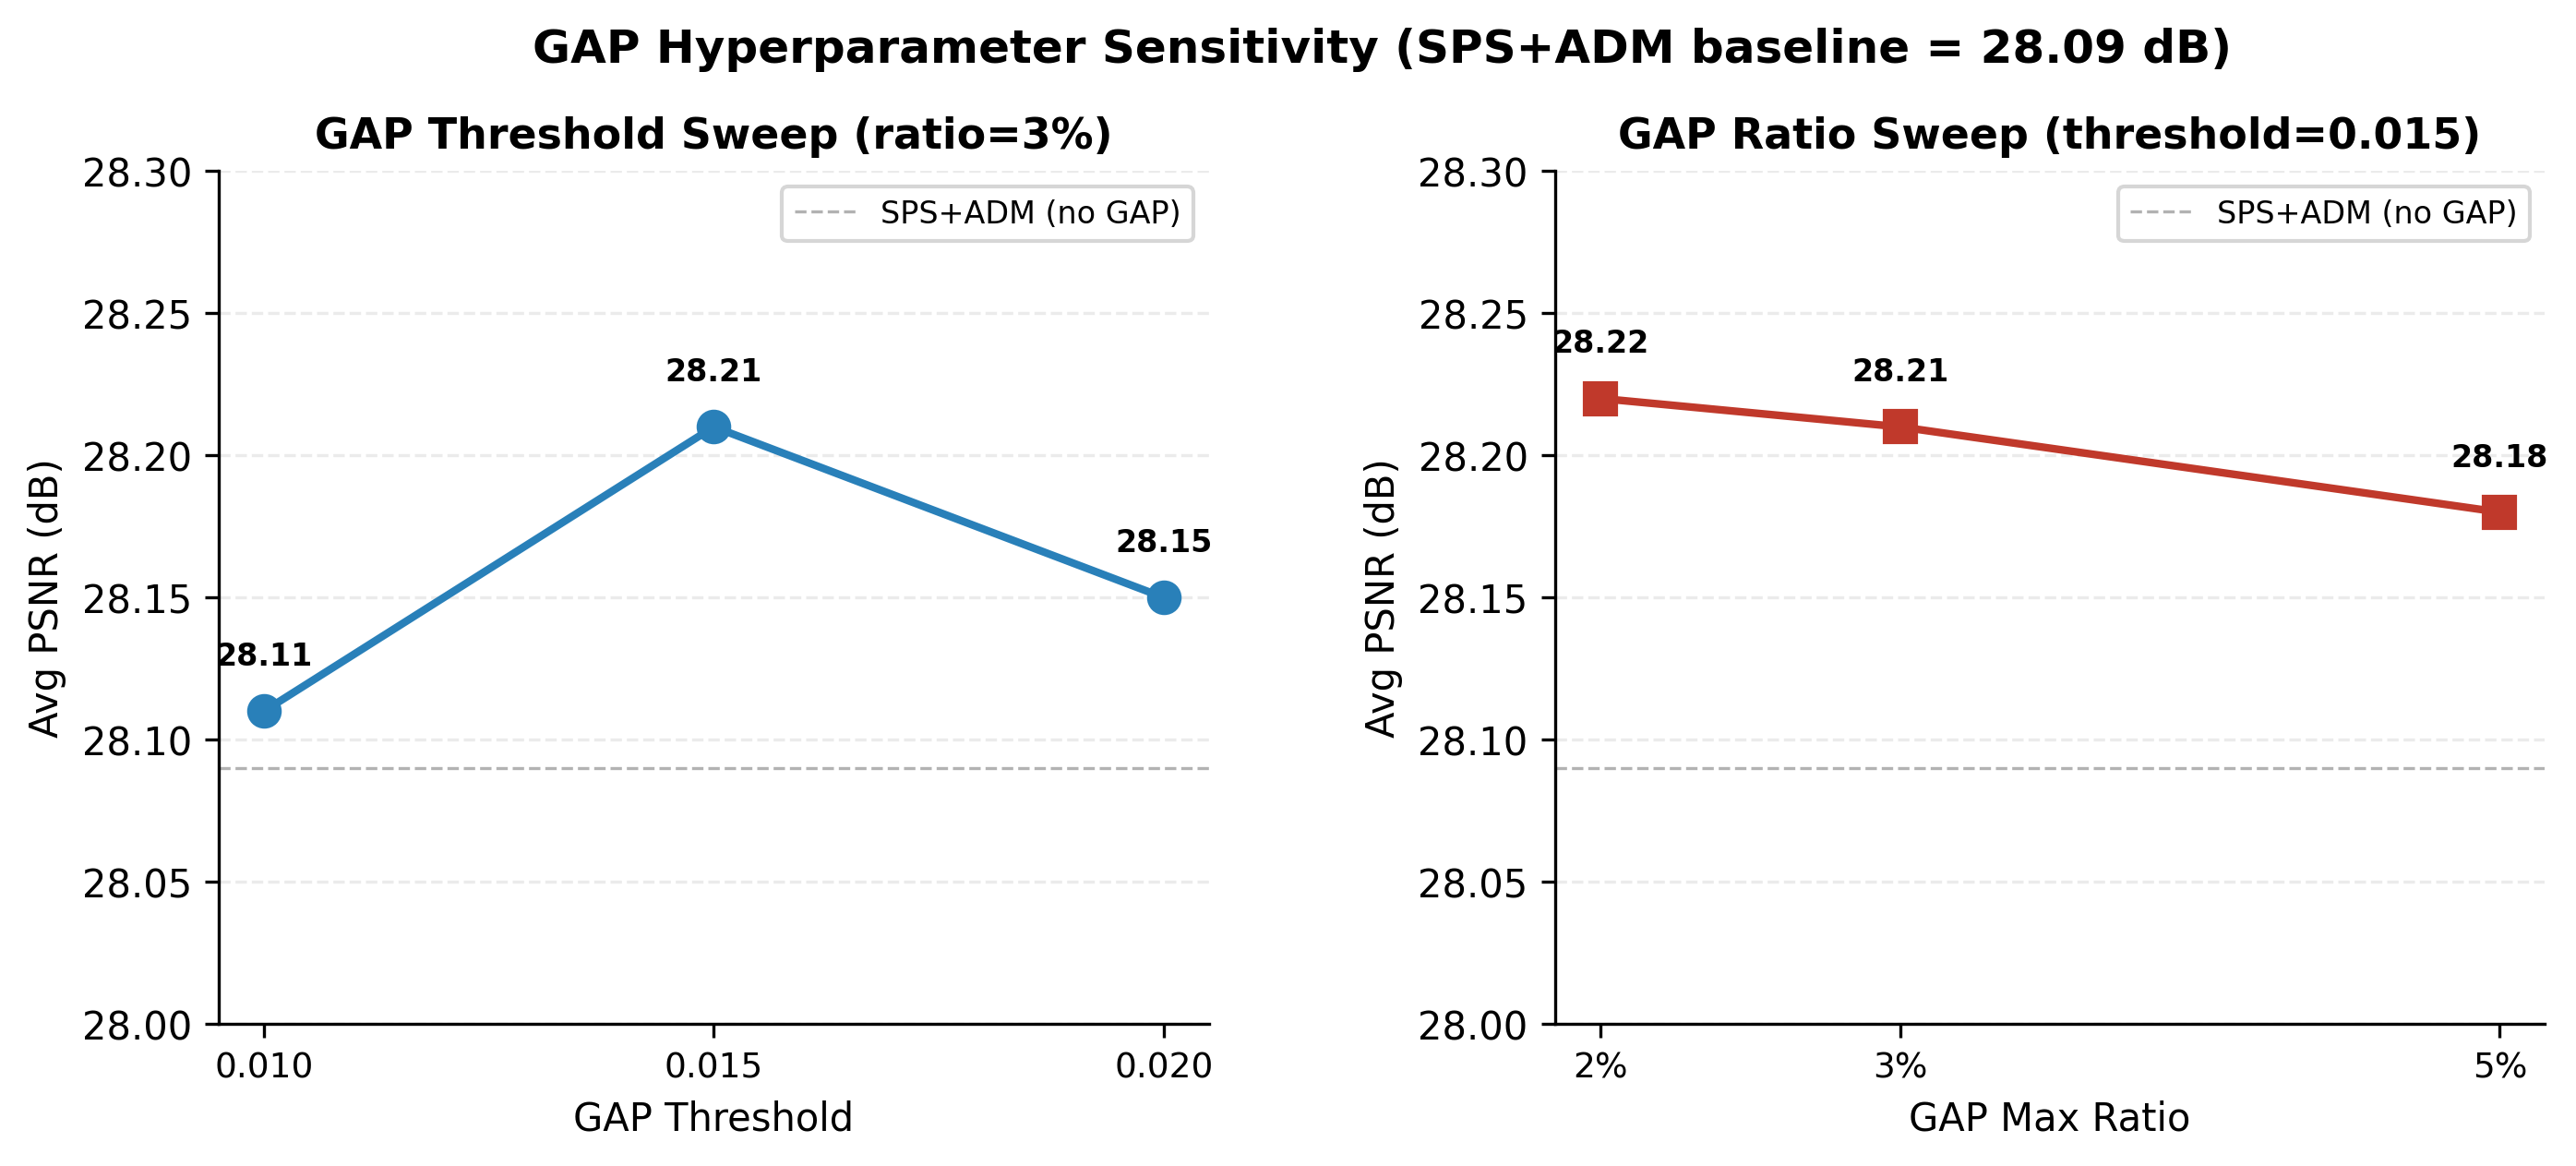
\includegraphics[width=\columnwidth]{../figures/fig_gap_sweep.png}
\caption{\gap\ hyperparameter sweep. Optimal threshold is 0.015 with ratio 2--3\%. Higher thresholds (0.020) over-prune and hurt Head performance.}
\label{fig:sweep}
\end{figure}

% 4.5 Cross-view Analysis
\subsection{Cross-view Comparison}
\label{sec:cross}

\begin{table}[t]
\centering
\caption{Summary comparison across view settings (average PSNR over 5 organs).}
\label{tab:views}
\begin{tabular}{lcccc}
\toprule
\textbf{Method} & \textbf{2v} & \textbf{3v} & \textbf{4v} \\
\midrule
\rtwo & 21.33 & 27.83 & 29.13 \\
\textbf{\spags} & \textbf{21.44} & \textbf{28.22} & \textbf{29.20} \\
\midrule
$\Delta$ & +0.11 & \textbf{+0.39} & +0.07 \\
\bottomrule
\end{tabular}
\end{table}

Table~\ref{tab:views} summarizes the cross-view comparison. The trend reveals that \spags\ delivers the largest improvement at 3 views (+0.39 dB), which is the primary setting for sparse-view CT novel view synthesis. At 2 views, the extreme sparsity limits all methods. At 4 views, the additional information reduces the margin as the baseline already performs well. This validates our design: \spags\ is most beneficial in the challenging but practical sparse-view regime.

The view-dependent behavior also provides insight into the working mechanism of each module. At 2 views, the FDK reconstruction quality is poor (severe streaks), limiting \sps's ability to provide meaningful anatomical priors. \gap's pruning is also less effective because the total number of Gaussians is smaller (fewer dense iterations occur with only 2 projection angles). At 4 views, the baseline itself achieves high quality (29.13 dB), and the room for \gap's redundancy control is reduced. The 3-view setting represents the sweet spot: the FDK reconstruction is informative enough for \sps\ to provide useful priors, and the gradient signals from 3 projection angles create sufficient over-clustering for \gap\ to demonstrate its pruning advantage, while information remains limited enough that spatially-aware density modulation from \adm\ provides additional benefit.

\begin{figure}[t]
\centering
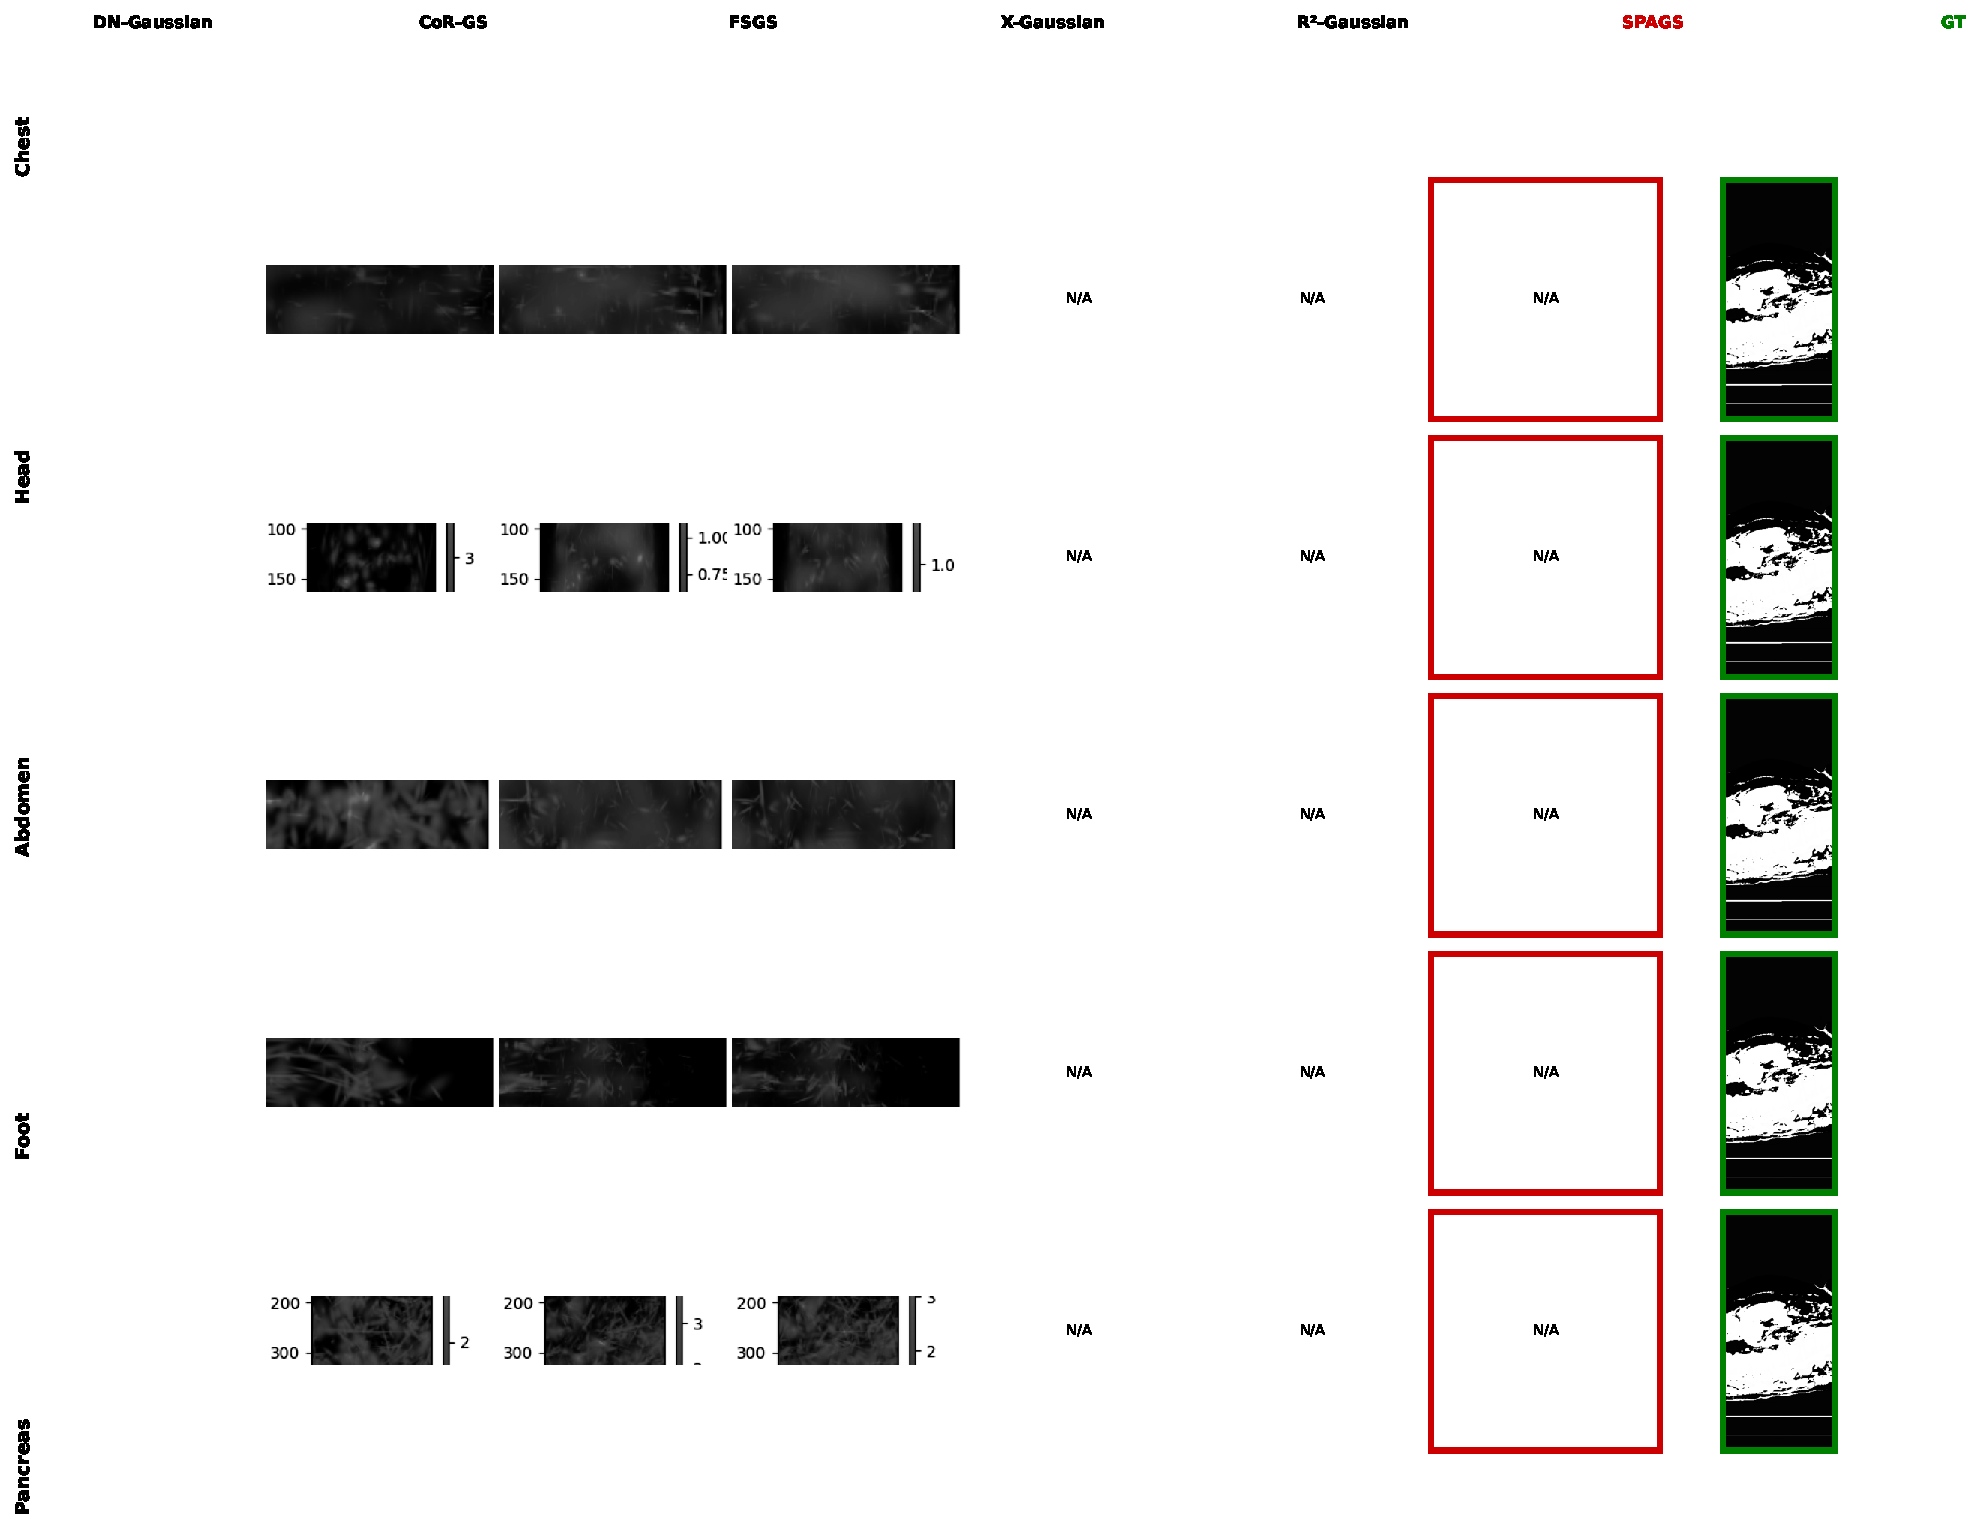
\includegraphics[width=\columnwidth]{../figures/fig_qualitative.pdf}
\caption{Qualitative comparison of rendered novel views at 4-view setting across 5 anatomical regions. \spags\ produces sharper anatomical boundaries and more accurate density contrast compared to baselines.}
\label{fig:qualitative}
\end{figure}

Figure~\ref{fig:qualitative} provides qualitative comparisons across all 5 organs. \spags\ consistently produces sharper anatomical boundaries and more accurate density contrast, particularly in challenging regions such as the Chest (lung boundaries) and Pancreas (small organ detail).

\subsection{Discussion and Limitations}
\label{sec:discussion}

Our experiments reveal several insights about the sparse-view CT NVS problem. First, the dominant contribution of \gap\ (+0.42 dB) compared to \sps\ (+0.21 dB) and \adm\ (+0.11 dB) suggests that \textit{controlling Gaussian redundancy} is the single most impactful intervention in this setting. This finding validates our core hypothesis that structural redundancy---not spatial sparsity---is the primary challenge in CT NVS, and that proximity-guided pruning is more effective than proximity-guided densification.

Second, the diminishing returns at 4 views (+0.07 dB) indicate that our spatial-aware approach provides the greatest benefit where information is most limited. As the number of projection views increases, the baseline optimizer receives sufficient gradient signal to overcome initialization bias and density estimation errors, reducing the need for explicit spatial priors. This trend is consistent with the behavior of learning-based methods in other sparse-view domains.

Third, we observe organ-specific sensitivity: the improvement is largest on Chest (+0.59 dB at 3 views) and Abdomen (+0.47 dB), which contain the most heterogeneous anatomy (bone-air-soft tissue interfaces). Conversely, Head and Foot show smaller improvements, likely because their denser, more uniform bone structures are already reasonably represented by the baseline. This suggests that \spags\ is most valuable for anatomical regions with high tissue contrast.

\textbf{Limitations.} Our method has several limitations that point to promising future directions. (1) The reliance on FDK reconstruction for initialization adds a preprocessing step ($<$1 second for a $128^3$ volume on GPU) that, while negligible, introduces a dependency on the TIGRE toolbox. (2) The K-planes resolution (64) and feature dimension (32) in \adm\ are fixed across all organs and view settings; optimal values may vary with anatomical complexity, and cross-organ adaptation could improve performance further. (3) Our evaluation is limited to fan-beam CT geometry with 2/3/4 views; extending to cone-beam and dynamic CT (4DCT) would test generalization across imaging protocols. (4) The current framework does not leverage learned priors from large CT datasets; integrating a pretrained denoising or reconstruction prior could provide additional regularization in the extreme sparse-view regime.

\subsection{Efficiency Analysis}
\label{sec:efficiency}

We analyze the computational cost of \spags\ relative to the \rtwo\ baseline. All experiments run on 2 RTX A6000 (48 GB) GPUs with 30,000 training iterations.

\textbf{Training time.} The \sps\ preprocessing (FDK reconstruction + density-weighted sampling) adds approximately 0.8 seconds per organ, a one-time cost before training. The \gap\ module adds KNN computation overhead during its active iterations (2K--20K, every 500 iterations): each proximity evaluation over $>$80K Gaussians takes $\sim$15 ms on GPU, totaling $\sim$0.5 seconds across the full training run. The \adm\ module adds forward and backward passes through the K-planes encoder and MLP, which amounts to $\sim$3 ms per iteration after warmup (15K--30K iterations), totaling $\sim$45 seconds. The overall training time of \spags\ is approximately 25--30 minutes per organ (depending on anatomy complexity), compared to 24--28 minutes for \rtwo, representing a modest $<$10\% overhead.

\textbf{Inference cost.} \spags\ introduces no additional overhead during inference. The final Gaussian count in \spags\ (80K--100K) is actually lower than \rtwo\ (100K--120K) due to \gap's pruning, resulting in slightly faster rendering ($\sim$12 ms vs $\sim$15 ms per projection at $256\times256$ resolution). The \adm\ K-planes encoder and MLP contribute $<1$ ms per forward pass and can be pre-computed after training.

Table~\ref{tab:efficiency} summarizes the computational cost breakdown. The total additional cost of \spags\ over \rtwo\ is less than 3 minutes per training run (about 10\% overhead), while inference is slightly faster due to the reduced Gaussian count. These results confirm that \spags\ is a practical framework that can be deployed in clinical workflows without significant computational burden.

\begin{table}[t]
\centering
\caption{Computational cost comparison between \rtwo\ and \spags. Times are averaged over 5 organs at 3-view setting.}
\label{tab:efficiency}
\begin{tabular}{lc}
\toprule
\textbf{Component} & \textbf{Time} \\
\midrule
\rtwo\ (baseline) training & 25 min \\
~~+ \sps\ preprocessing & $+$0.8 sec \\
~~+ \gap\ KNN computation (36 iterations) & $+$0.5 sec \\
~~+ \adm\ training (15K iterations) & $+$45 sec \\
\midrule
\textbf{\spags\ total training} & \textbf{$\sim$26 min} \\
\rtwo\ inference (per projection) & 15 ms \\
\textbf{\spags\ inference (per projection)} & \textbf{12 ms} \\
\bottomrule
\end{tabular}
\end{table}

% ============================================================
\section{Conclusion}
\label{sec:conclusion}
% ============================================================

This paper addresses the problem of sparse-view CT novel view synthesis by introducing explicit spatial awareness into the 3D Gaussian Splatting pipeline. Our core insight is that the primary challenge in CT NVS is not spatial sparsity---the standard focus of few-shot 3DGS---but structural redundancy, and that each stage of the 3DGS pipeline (initialization, densification, density optimization) requires spatial reasoning tailored to the unique characteristics of CT anatomy.

We operationalize this insight through three technical contributions: \sps\ (FDK-guided density-weighted initialization), \gap\ (proximity-guided pruning with gradient-aware filtering), and \adm\ (K-planes-based spatially-aware density modulation). On 5 organs across 2/3/4 projection views, \spags\ achieves an average PSNR of 28.22 dB at 3 views---a decisive +0.39 dB over \rtwo---and surpasses other state-of-the-art methods by 4--8 dB, with less than 10\% training overhead and zero inference cost. Ablation studies confirm that \gap's redundancy control is the single most impactful intervention (+0.42 dB), validating our core hypothesis about the nature of the CT NVS challenge.

A current limitation is that our K-planes parameters in \adm\ are fixed across organs and view settings; cross-organ adaptation could improve performance further. Extending \spags\ to dynamic CT (4DCT) and integrating learned denoising priors from large CT datasets are important next steps toward fully automated clinical deployment.

% ============================================================
\balance
\bibliography{references}
% ============================================================

\end{document}
